\chapter{Background Modeling}
\label{chap:modeling}

The study dedicated to the modeling of the major background is shown in this chapter.
The V+jets, which is the dominant background in all three lepton channel, has a knownissue of mismodeling. 
The reweighting is applied to the V+jet background sample, as described in the following sections.
Similar reweighting procedure is applied in all three lepton channels. Details are shown in 2-lepton channel hereafter.

\section{$m_{jj}^{tag}$ reweighting}
Figure~\ref{fig:2lep_mtag_before_rw} shows the $m^{tag}_{jj}$ distributions in CR of merged and resolved selection in 2-lepton channel.
The mis-modelling is seen as a slope in the ratio of data/MC in both regions.
These discrepancies have been known in the previous analysis round, as well as in other ATLAS analyses. 
This effect is believed to be related to the theoretical calculation of the collinear jets.
The reweighting is applied to the V+jets background sample to compensate this mis-modeling before defining the SRs and CRs. 
A simple linear fit is perfomed to the ratio between V+jets MC and the observed data in $m^{tag}_{jj}$ distribution, in each V+jets CRs. 

The fit function is defined as:
\begin{equation}
\label{eqn:reweight}
R=p_{0} * m_{jj}^{tag}+p_{1}
\end{equation}
where the R = $\frac{\mathrm{data}}{\mathrm{MC}}$. 
The fitting and the correction is performed only for the V+jets samples, therefore the other MC samples are subtracted at first. 
The all samples of mc16a+d+e period, same period as the full Run-2 dataset, is used for deriving the reweighting function, since there is no much difference in fitted value between mc periods when fitted each period separately. 
Both distributions are first normalized then the correction function (\ref{eqn:reweight}) is derived. 
In figure~\ref{}, the fitted line as a function of $m^{tag}_{jj}$ is shown. 
Each bin is defined to include at least 100 Z+jets events in order to have less than 5~\% statistical uncertainty. 
In merged control region, due to the large statistic difference between the low mass region and the high mass region, the barycenter of each bin is used as a fitting point, while in resolved region the bin center is used.

The estimated reweighting factor is applied as the event-by-event weight. 
Only the difference of the shape is corrected by this reweighting procedure, and difference of the normalization is accounted in the final fitting.
The reweighting function is subtracted in each control regions, then applied to the signal regions as weight.
The fitted parameter is summarized in the Table~\ref{tab:fit}. 
The reweighted distributions are shown in Figure~\ref{fig:2lep_mtag_before_rw}.

\begin{table}[htbp]
 \footnotesize
\begin{center}
\begin{tabular}{ | c | c | c |}
\hline
Parameter & Merged CRVjet & Resolved CRVjet  \\
\hline
$p_{0}$ (slope) [$\GeV^{-1}$] & $(-23.8 \pm 2.5)e^{-5}$ &  $(-17.5 \pm 0.5)e^{-5}$ \\
 \hline
$p_{1}$ (constant)  & $1.298 \pm 0.031$ & $1.187 \pm 0.005$ \\
\hline
\end{tabular}
\caption{\label{tab:fit} Fitted re-weighting parameters for the merged and resolved regions. The errors written here are the uncertainties of the fitted parameters. }
  \end{center}
\end{table}


\begin{figure}[ht]
    \centering
    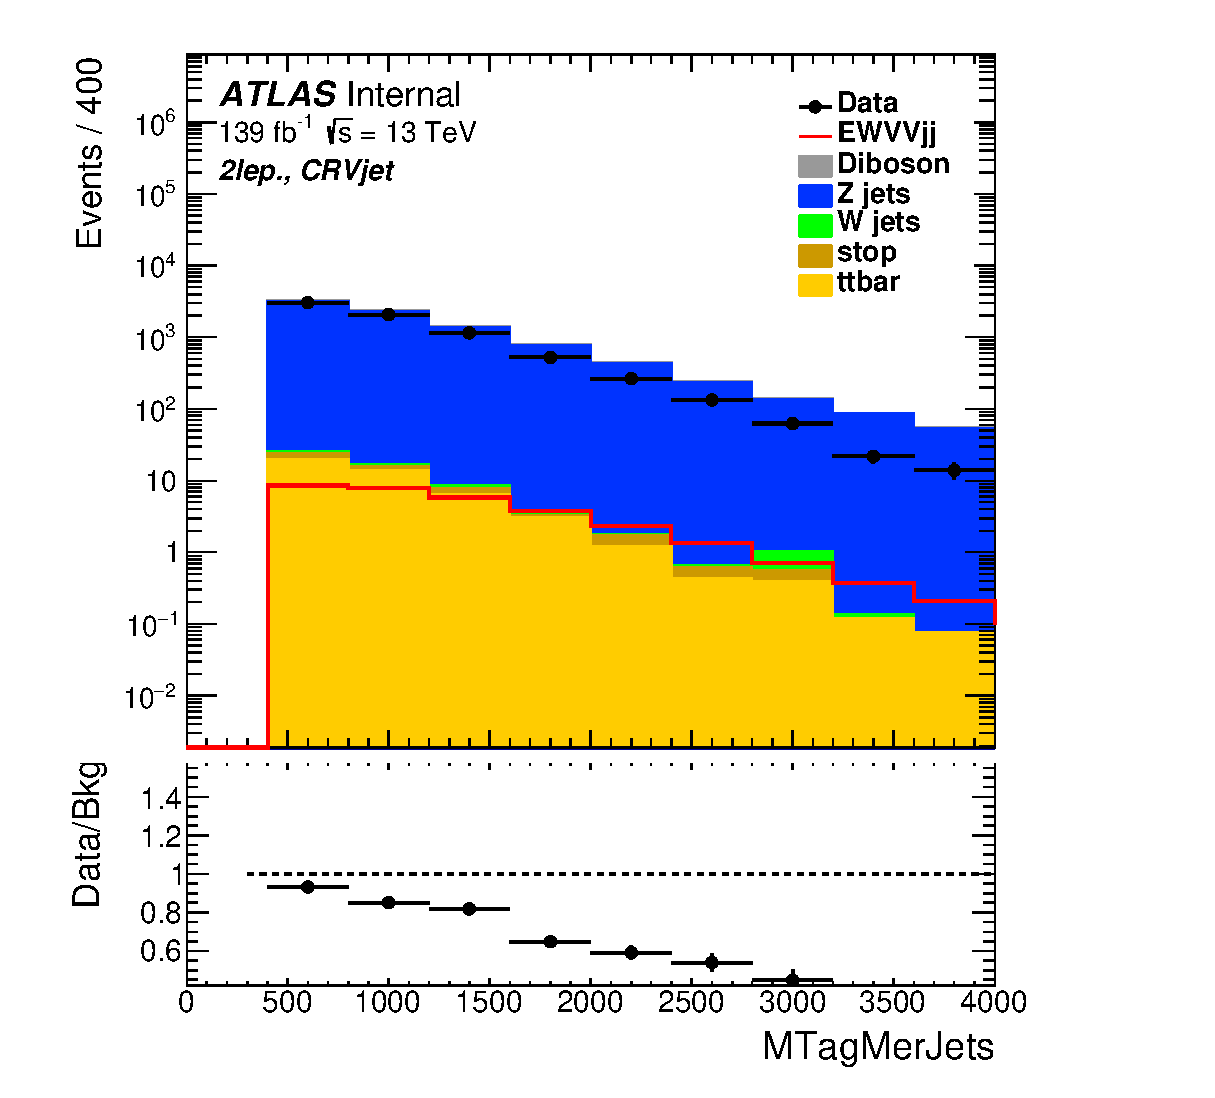
\includegraphics[width=0.45\textwidth]{figures/2lep/reweighting/before_reweighting/C_0ptag1pfat0pjet_0ptv_CRVjet_MTagMerJets_Log.eps}
    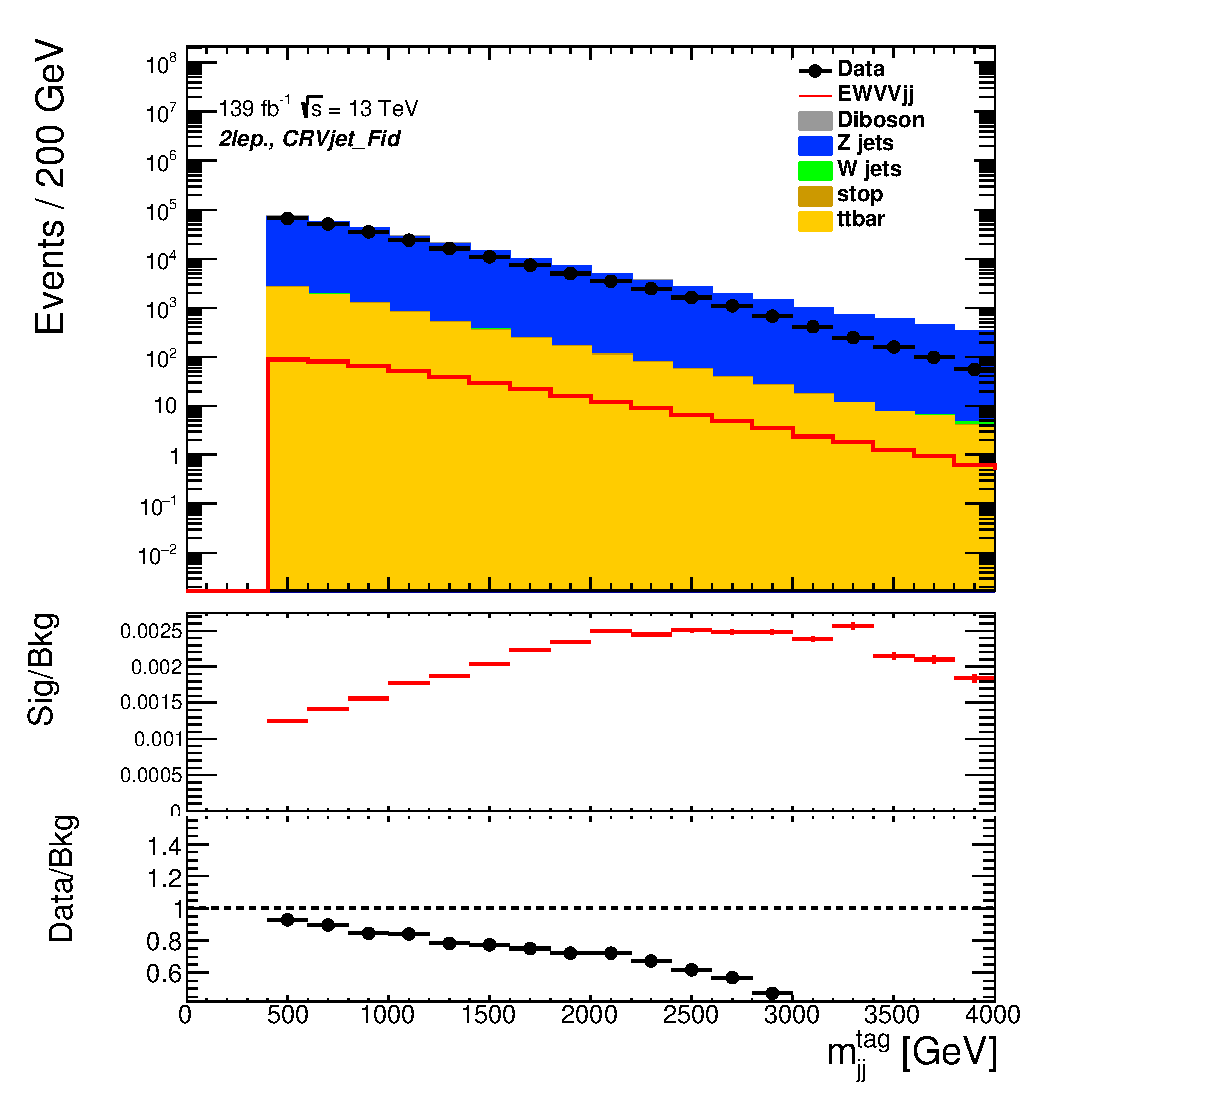
\includegraphics[width=0.45\textwidth]{figures/2lep/reweighting/before_reweighting/C_0ptag2pjet_0ptv_CRVjet_Fid_MTagResJets_Log.eps}
    \caption{ $m^{tag}_{jj}$ distributions before applying reweighting for the merged (a) and resolved (b) control regions in the 2-lepton channel.}
    \label{fig:2lep_mtag_before_rw}
\end{figure}

\begin{figure}[ht]
    \centering
    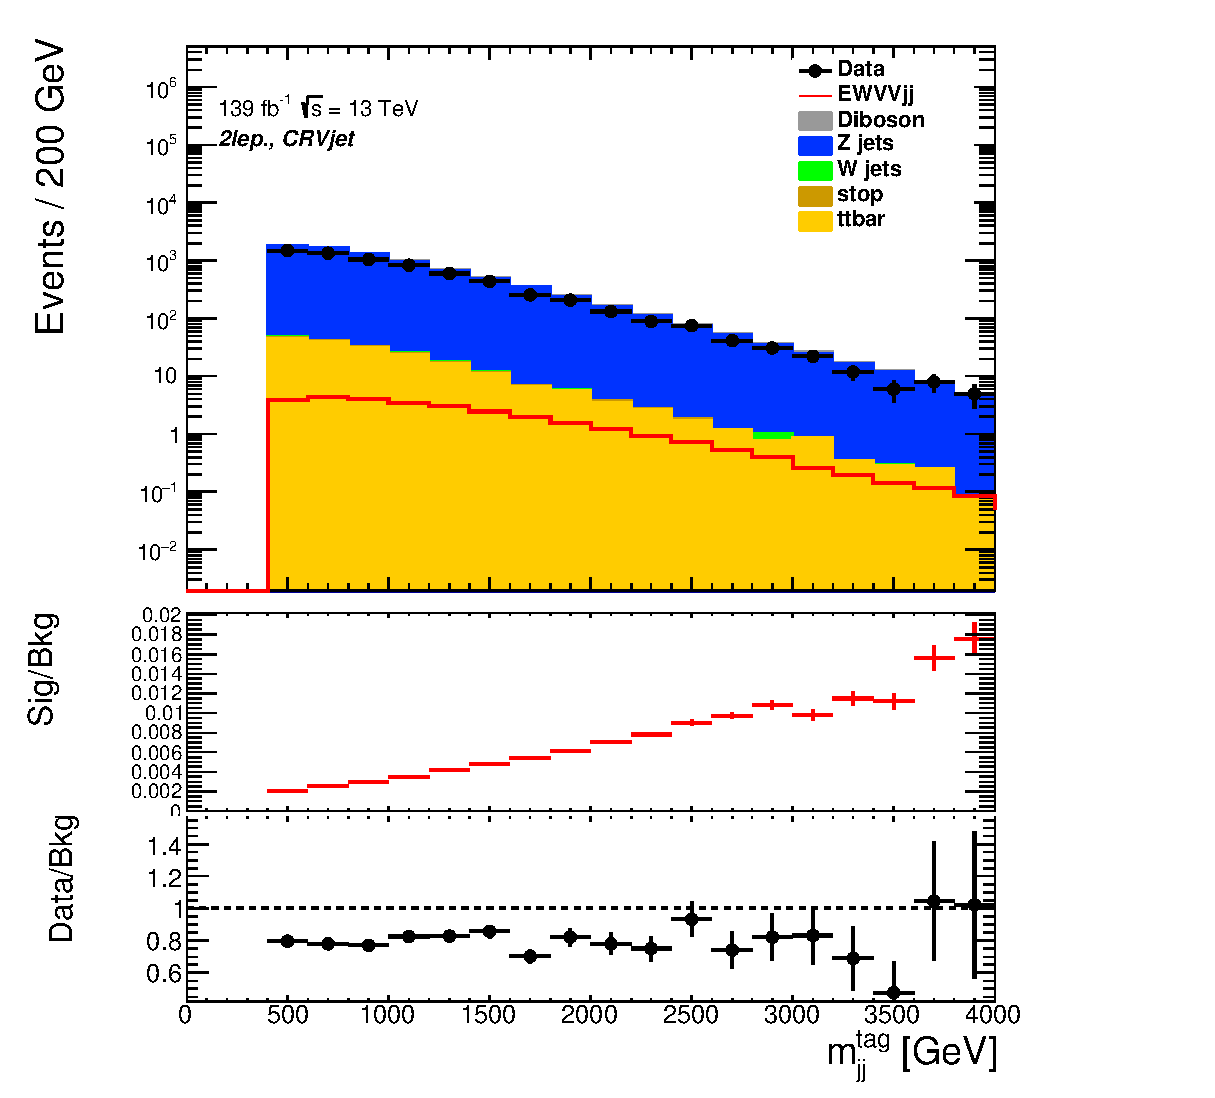
\includegraphics[width=0.45\textwidth]{figures/2lep/reweighting/after_reweighting/C_0ptag1pfat0pjet_0ptv_CRVjet_MTagMerJets_Log.eps}
    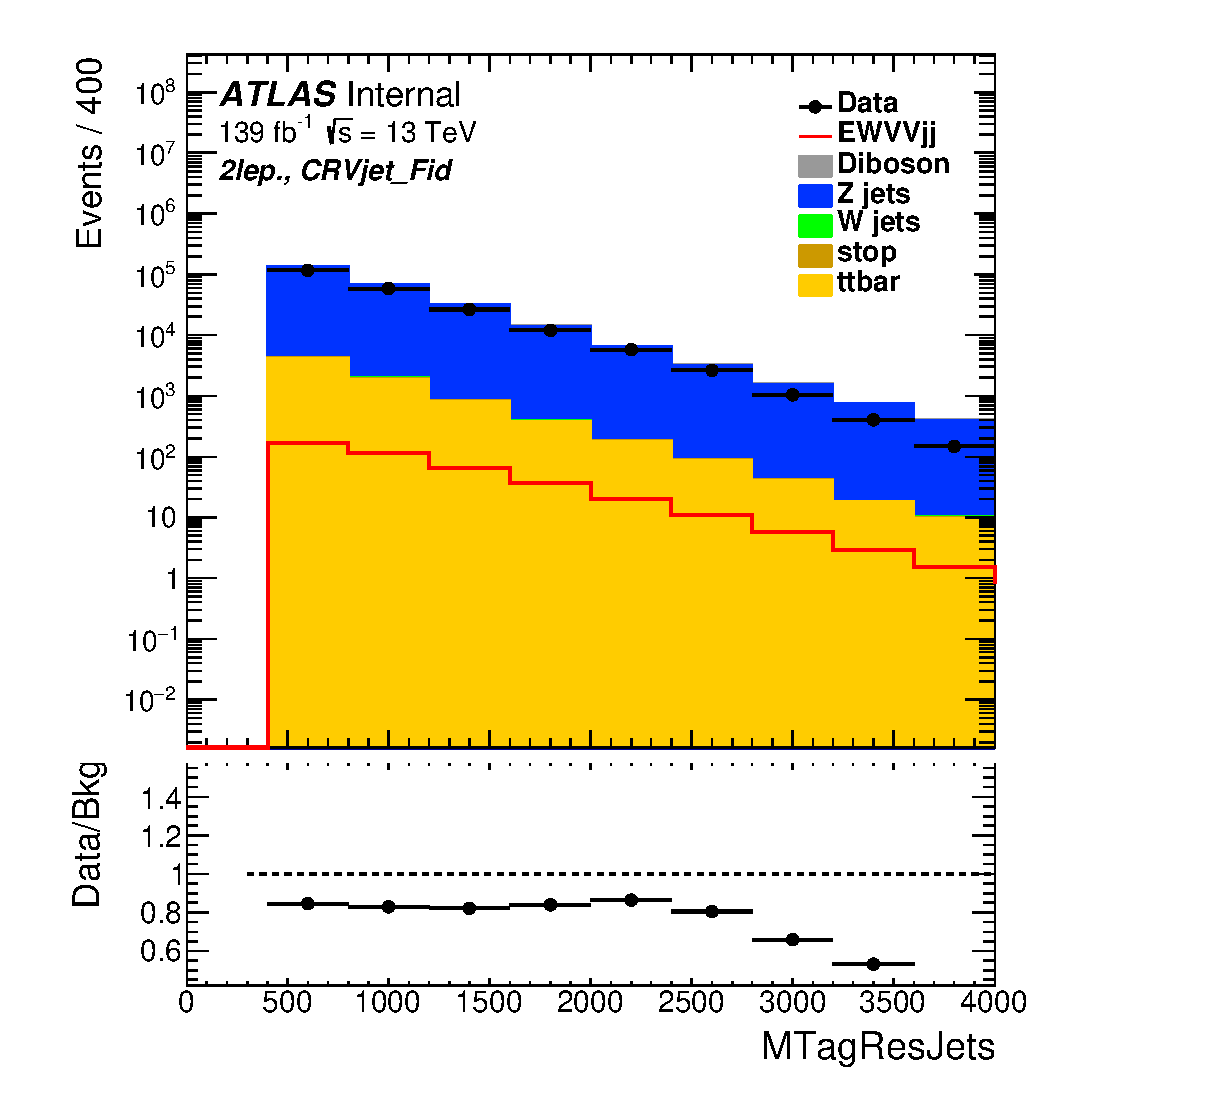
\includegraphics[width=0.45\textwidth]{figures/2lep/reweighting/after_reweighting/C_0ptag2pjet_0ptv_CRVjet_Fid_MTagResJets_Log.eps}
    \caption{ $m^{tag}_{jj}$ distributions after applying reweighting for the merged (a) and resolved (b) control regions in the 2-lepton channel. The slope seen before reweighting is corrected in the Z+jet CR.}
    \label{fig:2lep_mtag_before_rw}
\end{figure}

The comparison of distributions from data and MC for various kinematic variables after reweighting in the 2-lepton Z+jets merged and resolved control region are shown in Figure \ref{fig:2lep_zjets_merged_CR} and Figure \ref{fig:2lep_zjets_resolved_CR}
respectively. The data/MC ratios are flat, indicating the successfull reweighting.

% 2-lepton new merged CR - plots
\begin{figure}[ht]
 \centering
   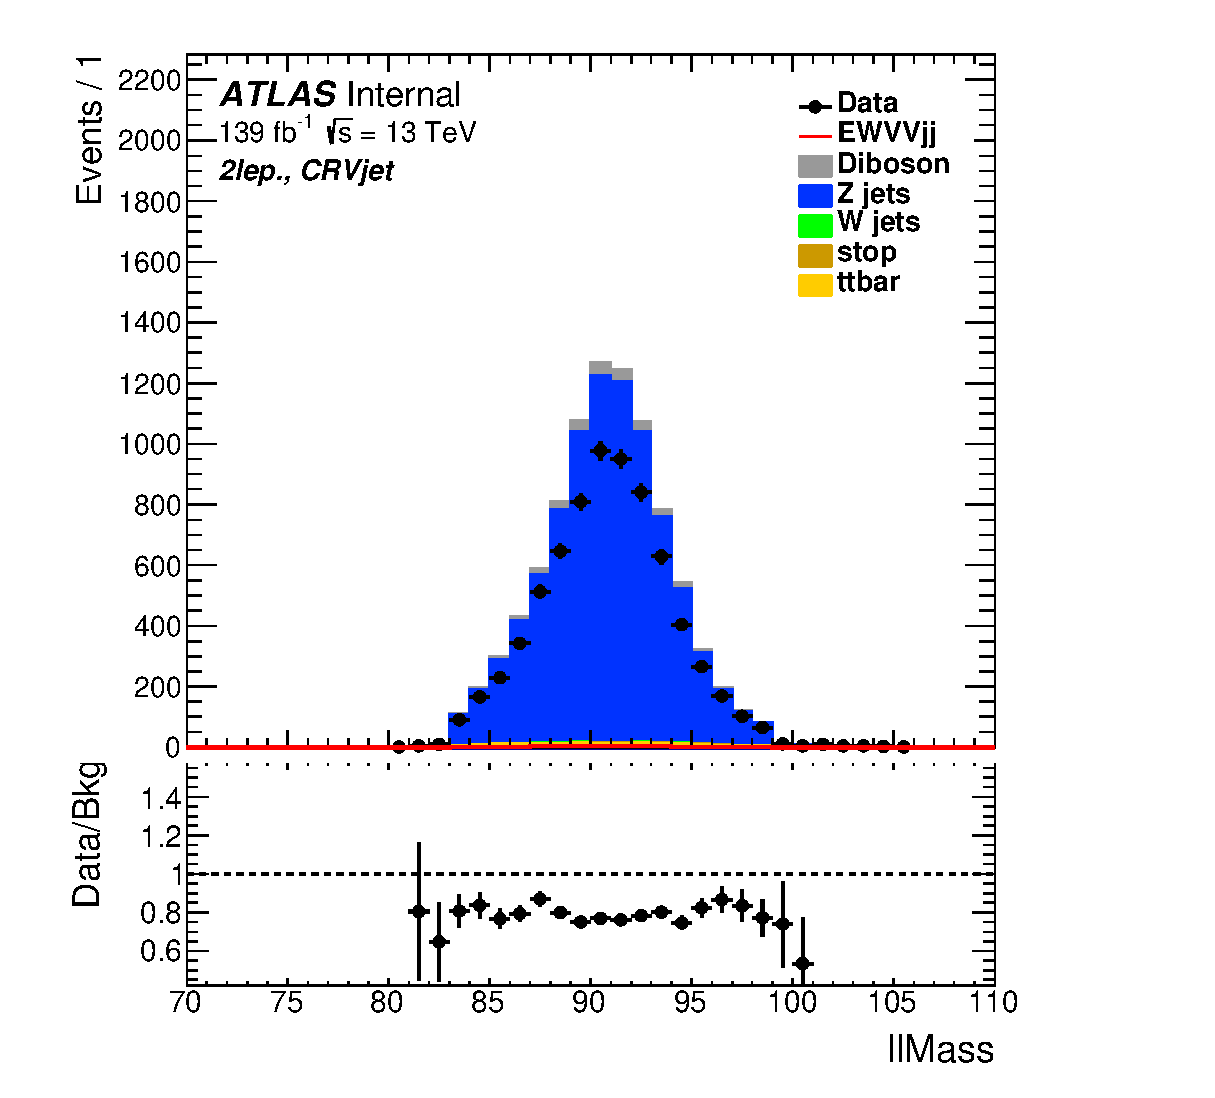
\includegraphics[width=0.30\textwidth]{figures/2lep/reweighting/after_reweighting/C_0ptag1pfat0pjet_0ptv_CRVjet_llMass_Lin.eps}
   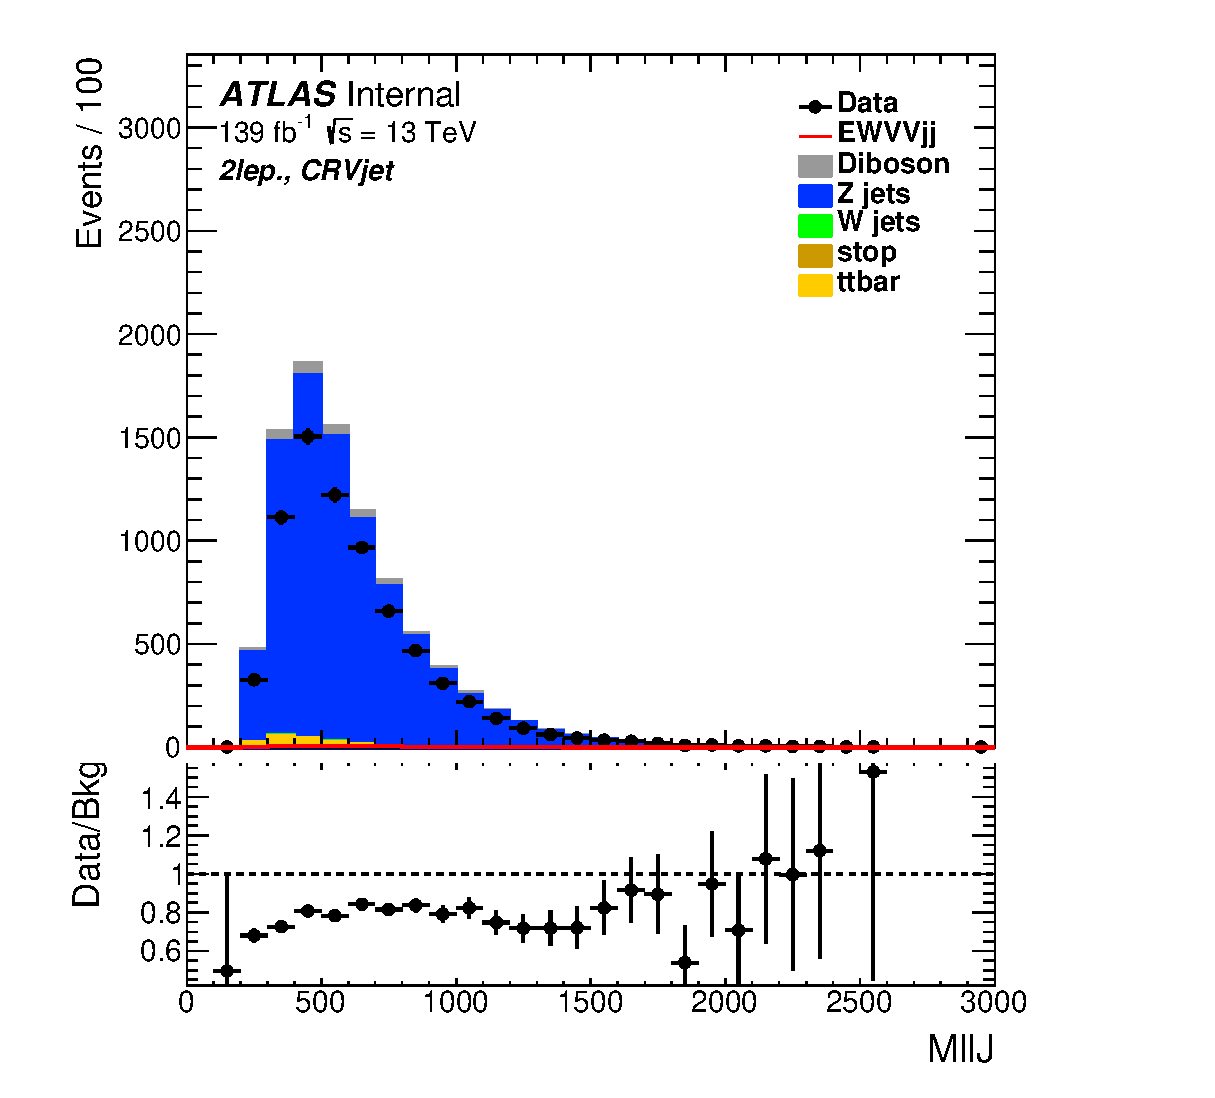
\includegraphics[width=0.30\textwidth]{figures/2lep/reweighting/after_reweighting/C_0ptag1pfat0pjet_0ptv_CRVjet_MllJ_Lin.eps}
   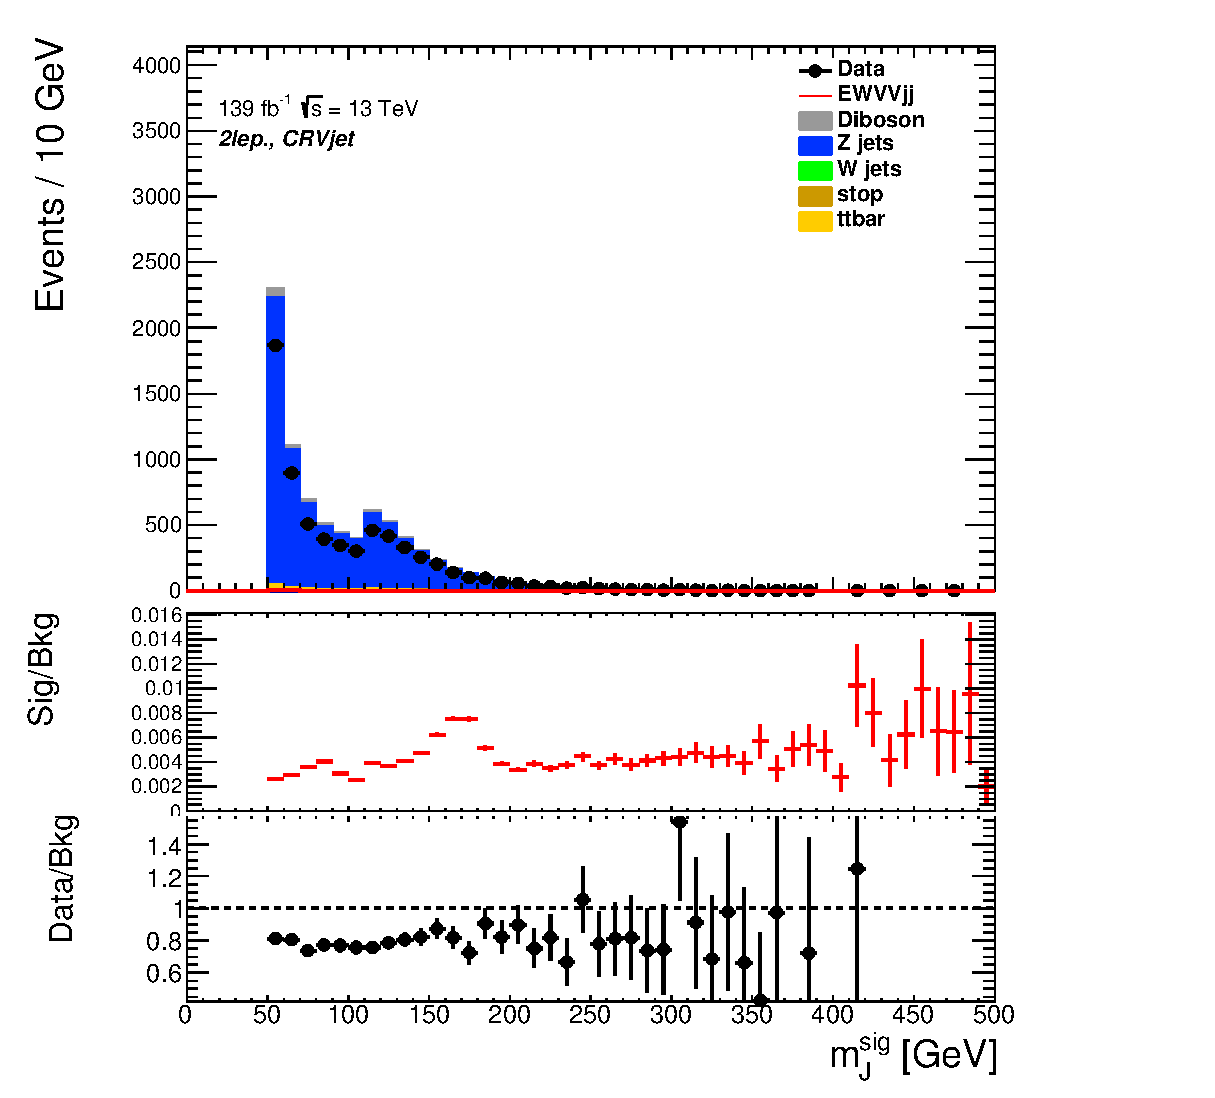
\includegraphics[width=0.30\textwidth]{figures/2lep/reweighting/after_reweighting/C_0ptag1pfat0pjet_0ptv_CRVjet_fatJetMass_Lin.eps}
    \caption{ Various kinematic variables in the Z+jets merged CR in the 2-lepton channel analysis.}
    \label{fig:2lep_zjets_merged_CR}
\end{figure}


% 2-lepton resolved CR fiducial- plots
\begin{figure}[ht]
    \centering
   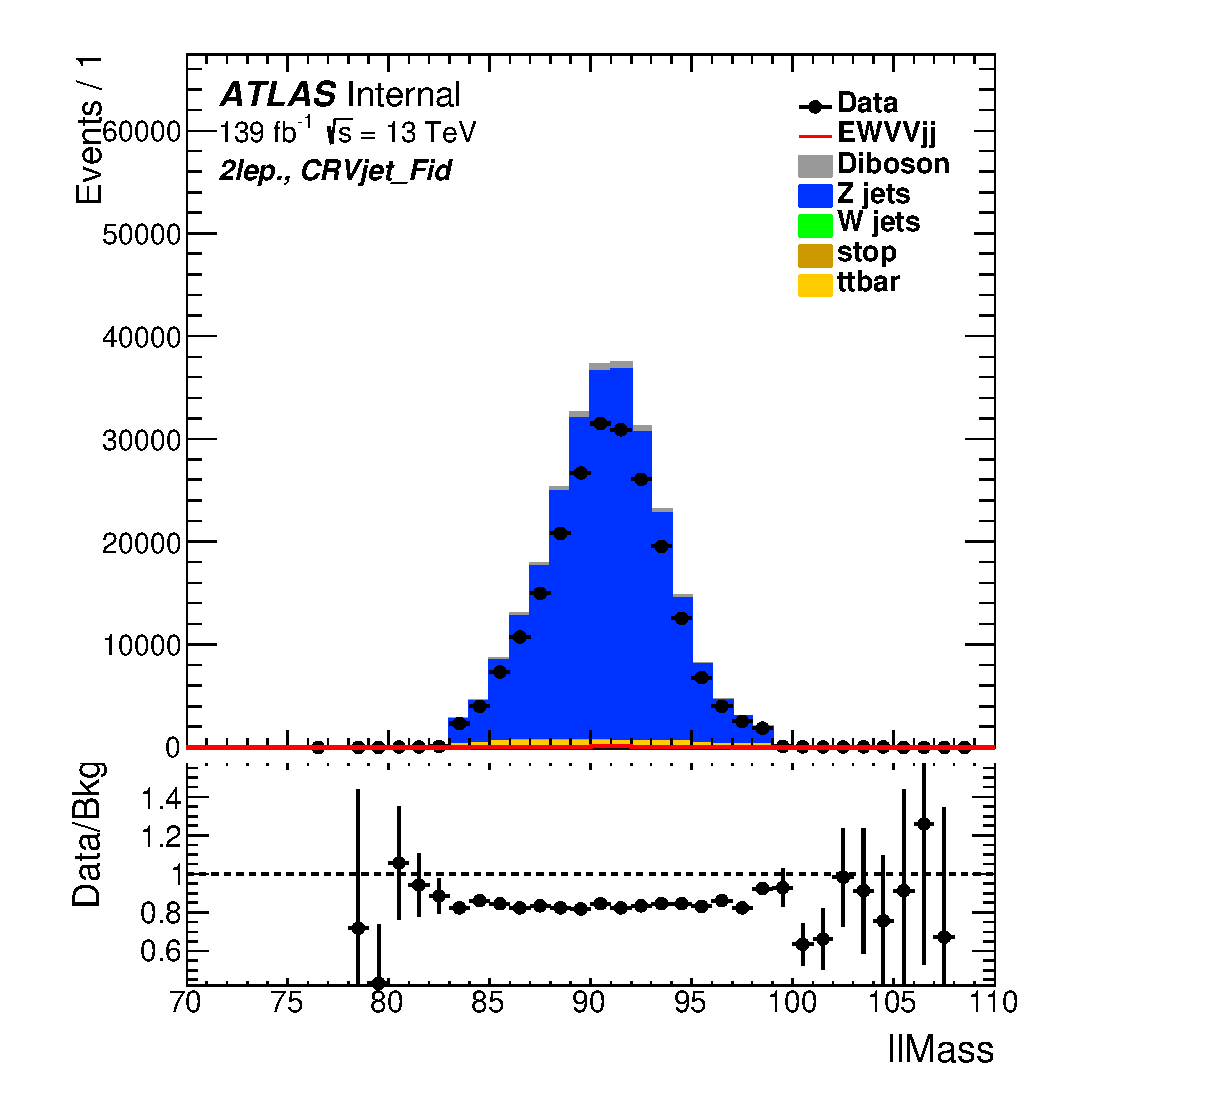
\includegraphics[width=0.30\textwidth]{figures/2lep/reweighting/after_reweighting/C_0ptag2pjet_0ptv_CRVjet_Fid_llMass_Lin.eps}
   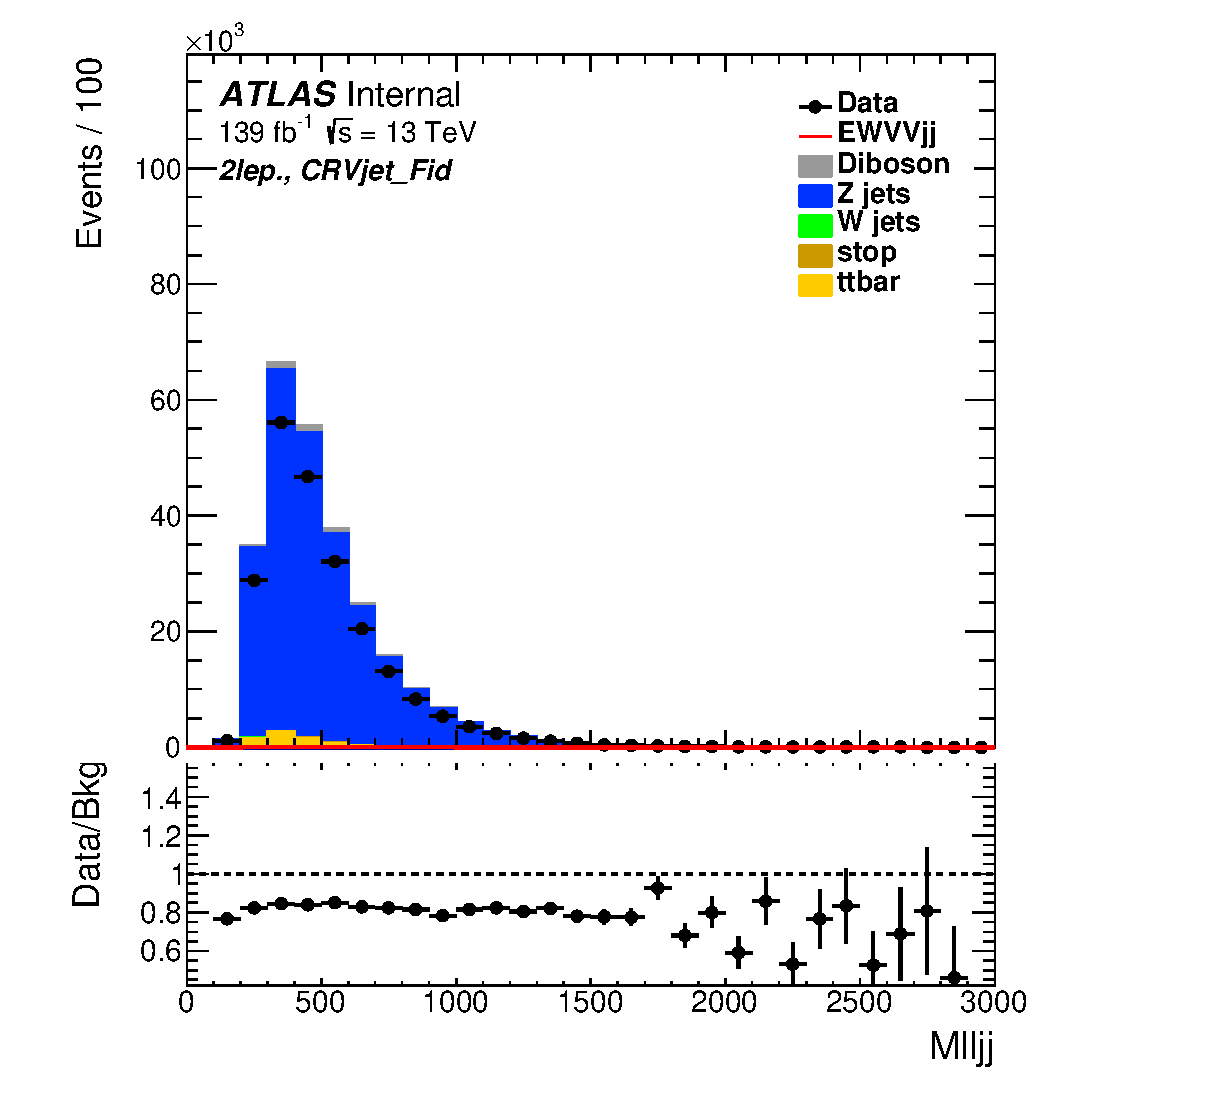
\includegraphics[width=0.30\textwidth]{figures/2lep/reweighting/after_reweighting/C_0ptag2pjet_0ptv_CRVjet_Fid_Mlljj_Lin.eps}
  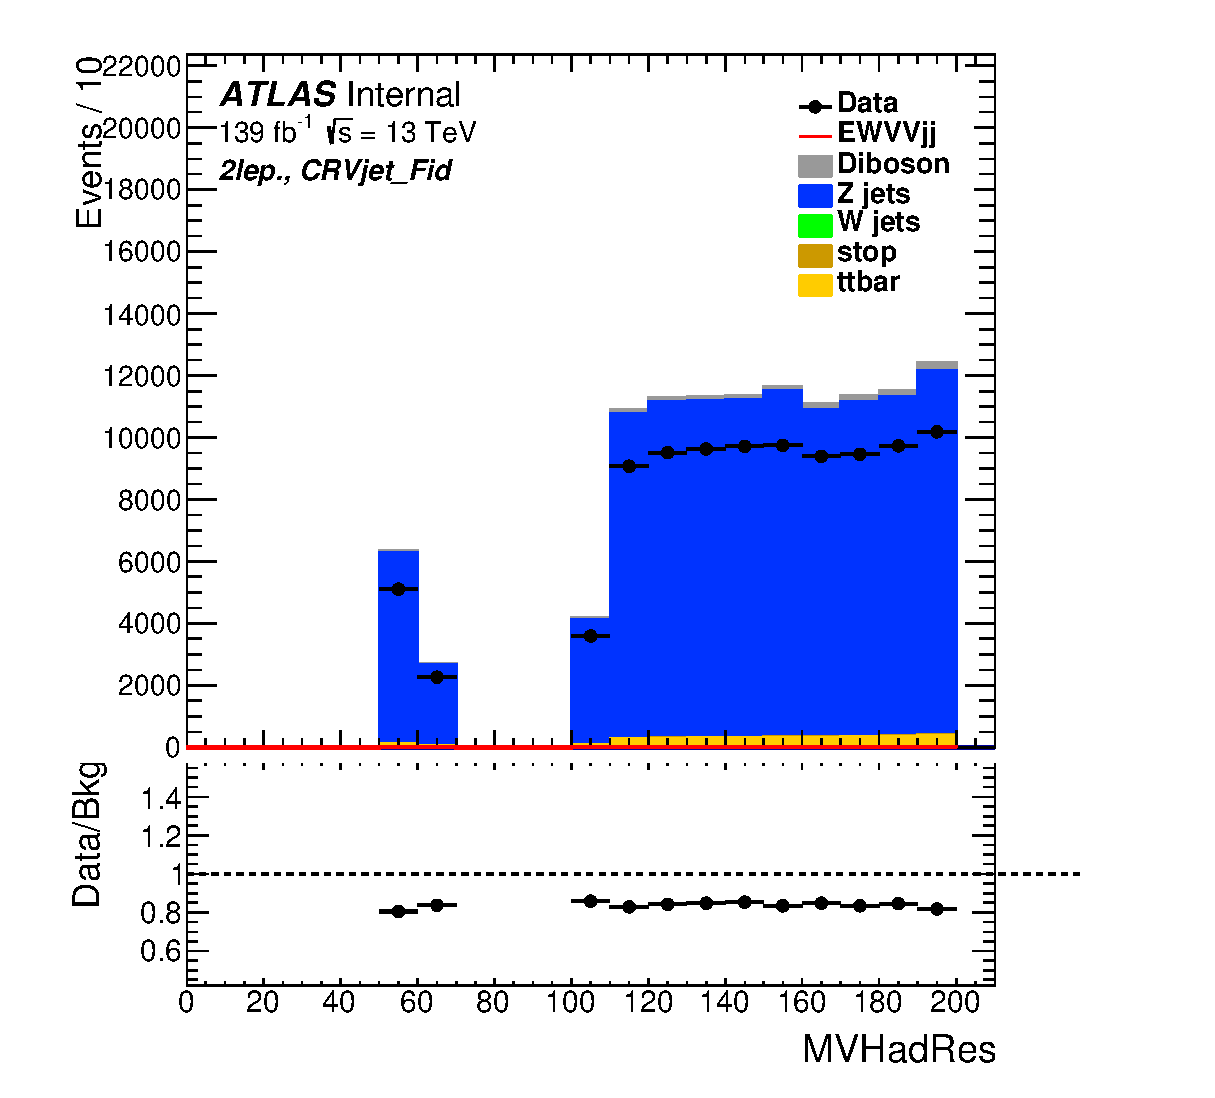
\includegraphics[width=0.30\textwidth]{figures/2lep/reweighting/after_reweighting/C_0ptag2pjet_0ptv_CRVjet_Fid_MVHadRes_Lin.eps}
  \caption{ Various kinematic variables in the Z+jets resolved CR in the 2-lepton channel analysis.}
   \label{fig:2lep_zjets_resolved_CR}
\end{figure}

%************write something about MadGraph and the dedicated modeling uncertainty here**********
There is alternative samples using MadGraph instread of Shelpa~2.2.1 as generator. 
The modeling of the MadGraph, as well as new version of Shelpa~2.2.11 samples in 2-lepton Z+jets CRs are shown in Figure~\ref{}. No reweight is applied here for comparing. Backgrounds are normalized to the data to see the shapes of the MC. 
This $m^{tag}_{jj}$ MadGraph has better modeling in our phase space which requires high $m^{tag}_{jj}$. However Shelpa is used as the baseline sample, since it has much statistics.
This difference between two generator is included in the final fitting as a theoretical uncertainty, discribed the detail in chapter~\ref{chap:systematic}.

$The reweighting is also applied in  the other lepton chnaaels. In 1-lepgon channel, the similar procedue 
